% =========================================================
% CONFIGURACION DEL DOCUMENTO
% =========================================================
\providecommand{\main}{..}
\documentclass[\main/main.tex]{subfiles}

% =========================================================
% CONTENIDO
% =========================================================
\begin{document}
\chapter{Código LabVIEW para Implementación}
\begin{landscape}

\begin{figure}
\begin{centering}
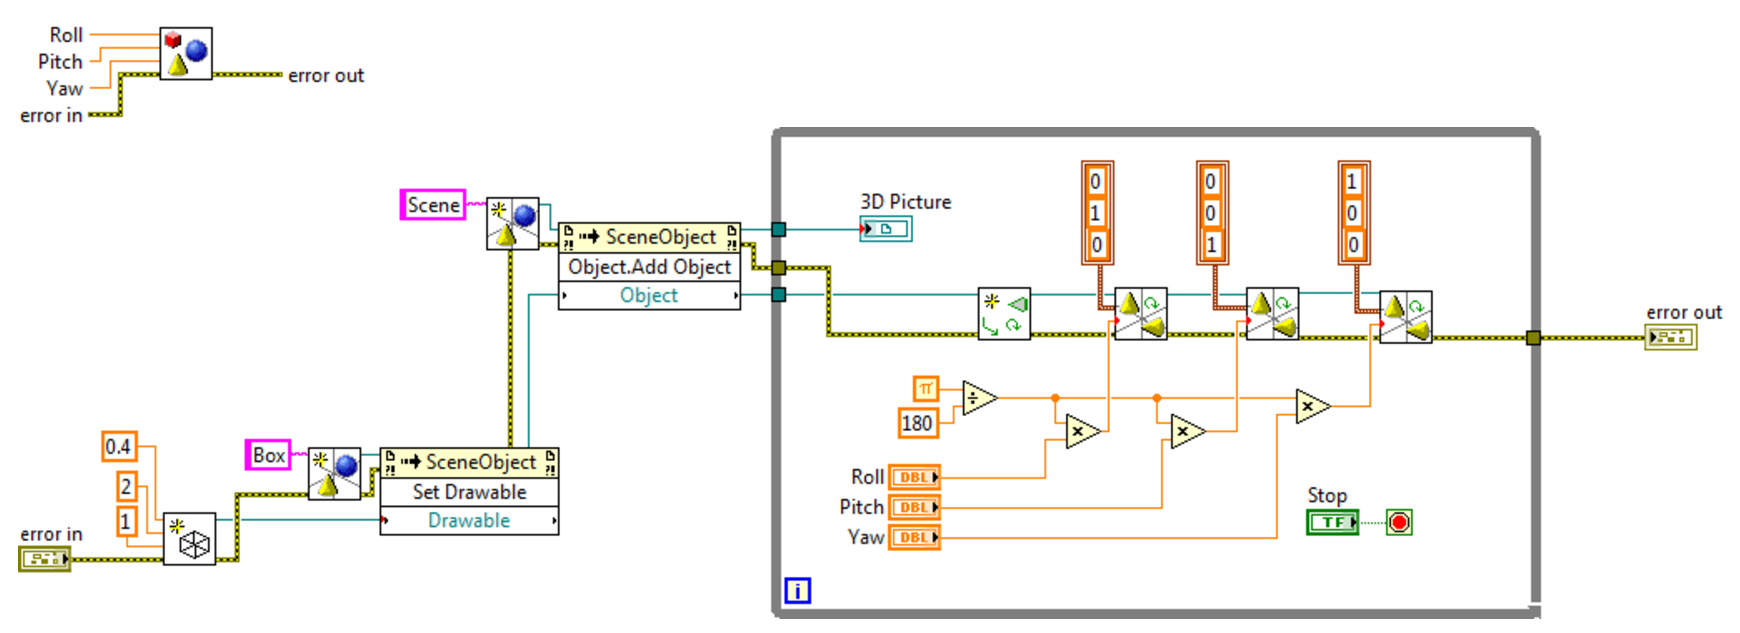
\includegraphics[scale=0.6]{3D_Picture}
\par\end{centering}
\caption{Visualización de medición de ángulos en 3D. Roll, Pitch y Yaw seteados
como variables compartidas.}
\end{figure}

\begin{figure}
\begin{centering}
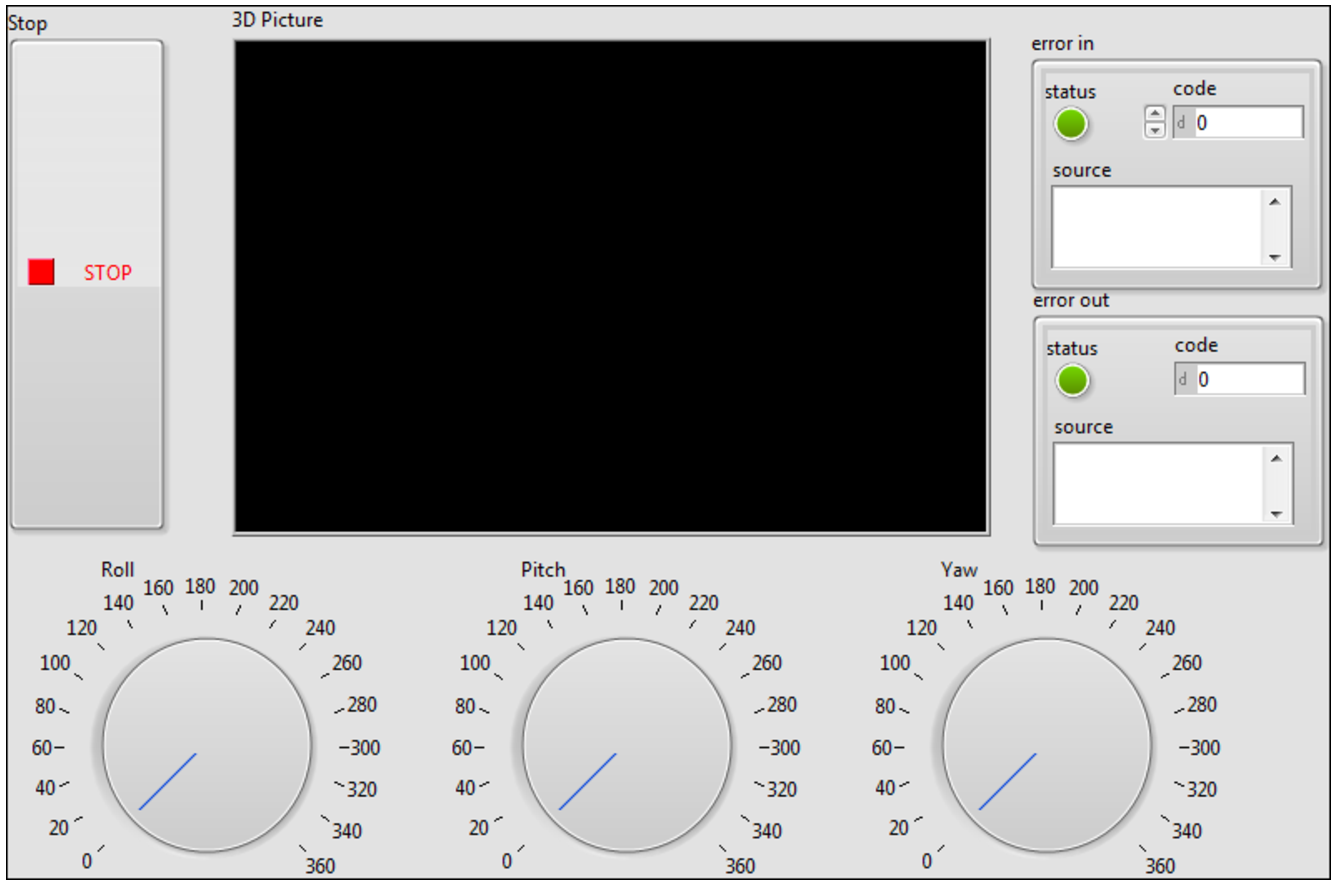
\includegraphics[scale=0.6]{3D_PicturePanel}
\par\end{centering}
\caption{Panel frontal simulación 3D para la medición de ángulos.}
\end{figure}

\begin{figure}
\begin{centering}
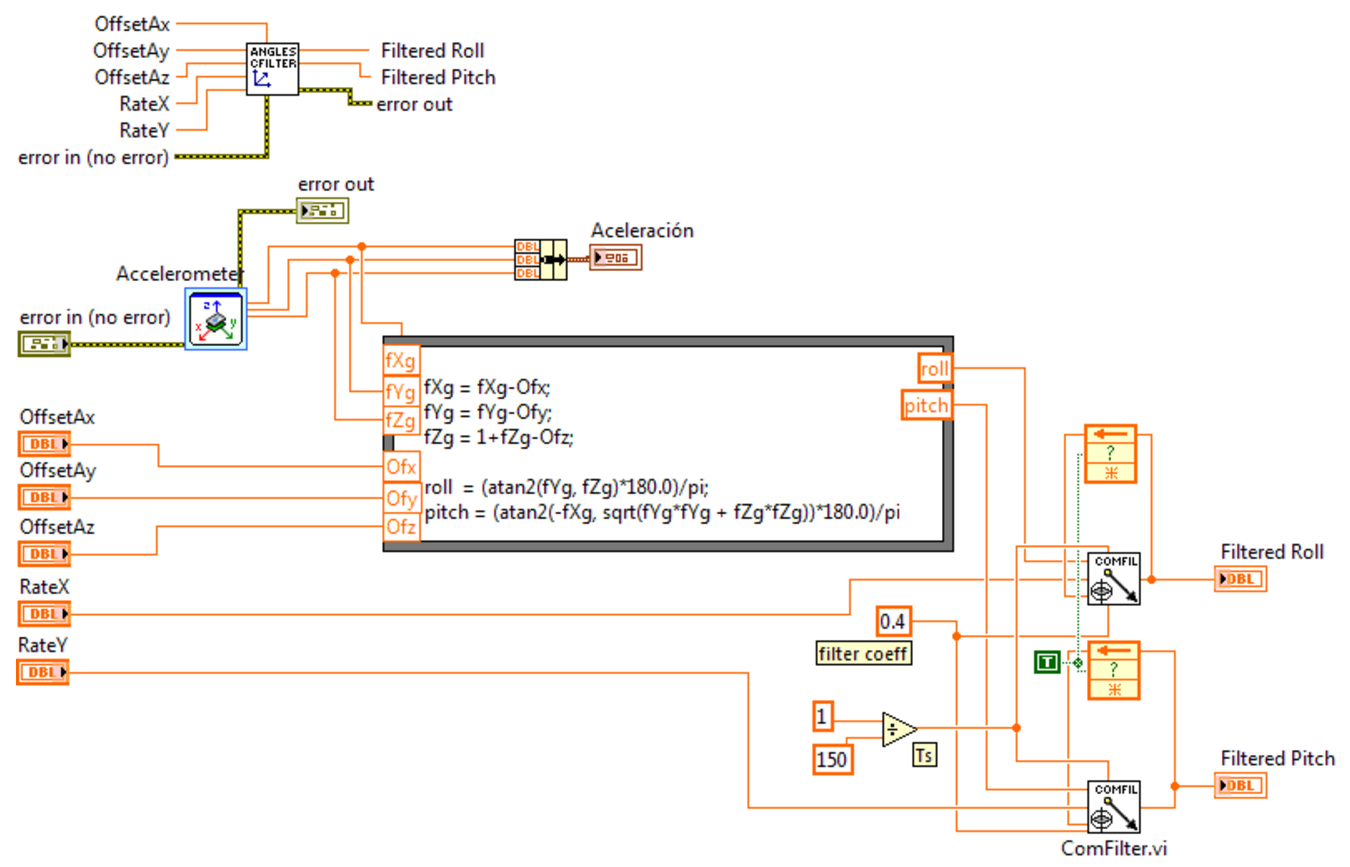
\includegraphics[scale=0.8]{AngPitchRoll}
\par\end{centering}
\caption{Calculo de ángulos Pitch y Roll con filtro complementario.}
\end{figure}

\begin{figure}
\begin{centering}
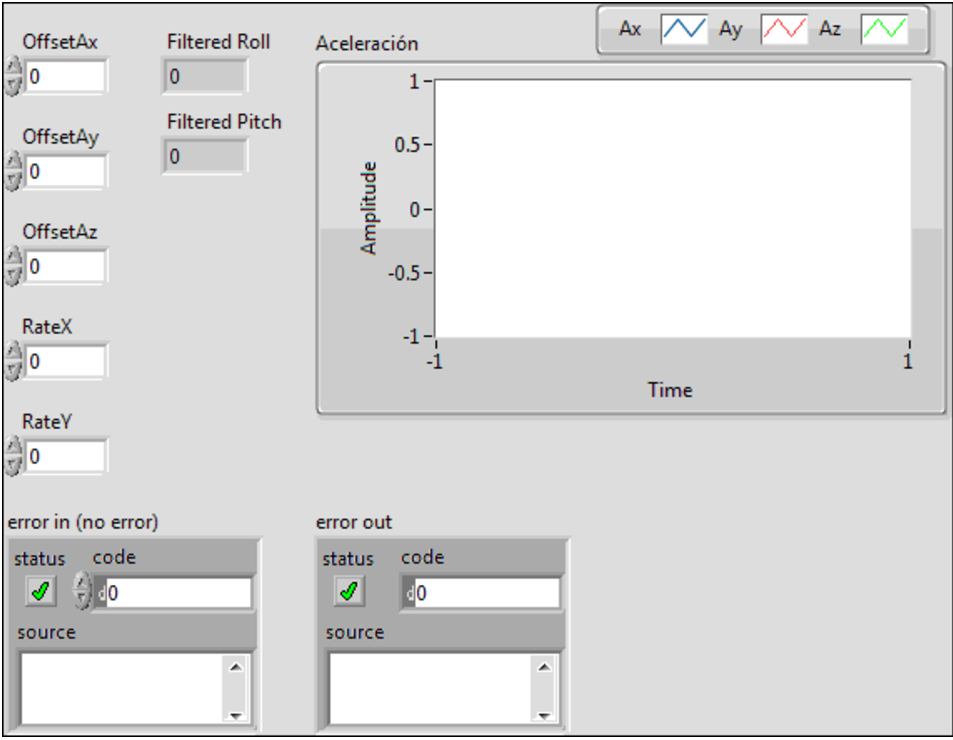
\includegraphics[scale=0.8]{AngPitchRollPanel}
\par\end{centering}
\caption{Panel frontal para visualización de ángulos Pitch y Roll con filtro
complementario.}
\end{figure}

\begin{figure}
\begin{centering}
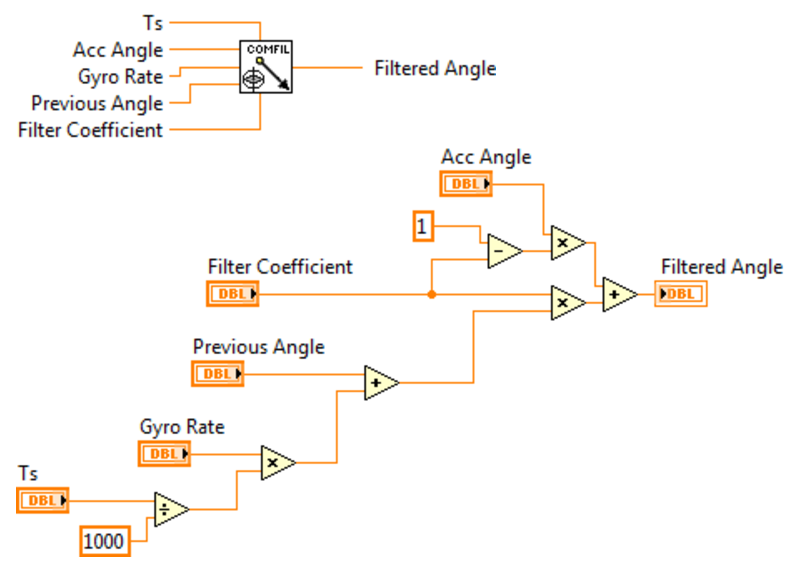
\includegraphics[scale=0.8]{ComFilter}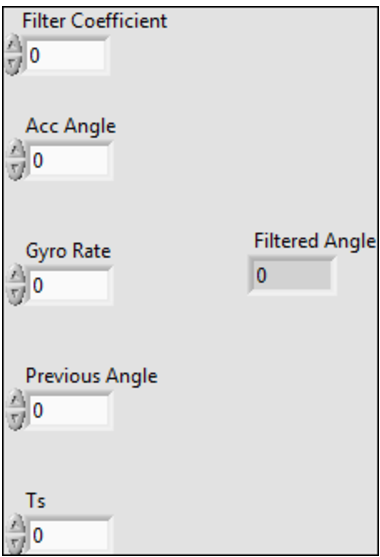
\includegraphics[scale=0.6]{ComFilterPanel}
\par\end{centering}
\caption{Filtro complementario para Pitch y Roll. Une medida de acelerómetro
y gyróscopo a través de ponderación.}
\end{figure}

\begin{figure}
\begin{raggedright}
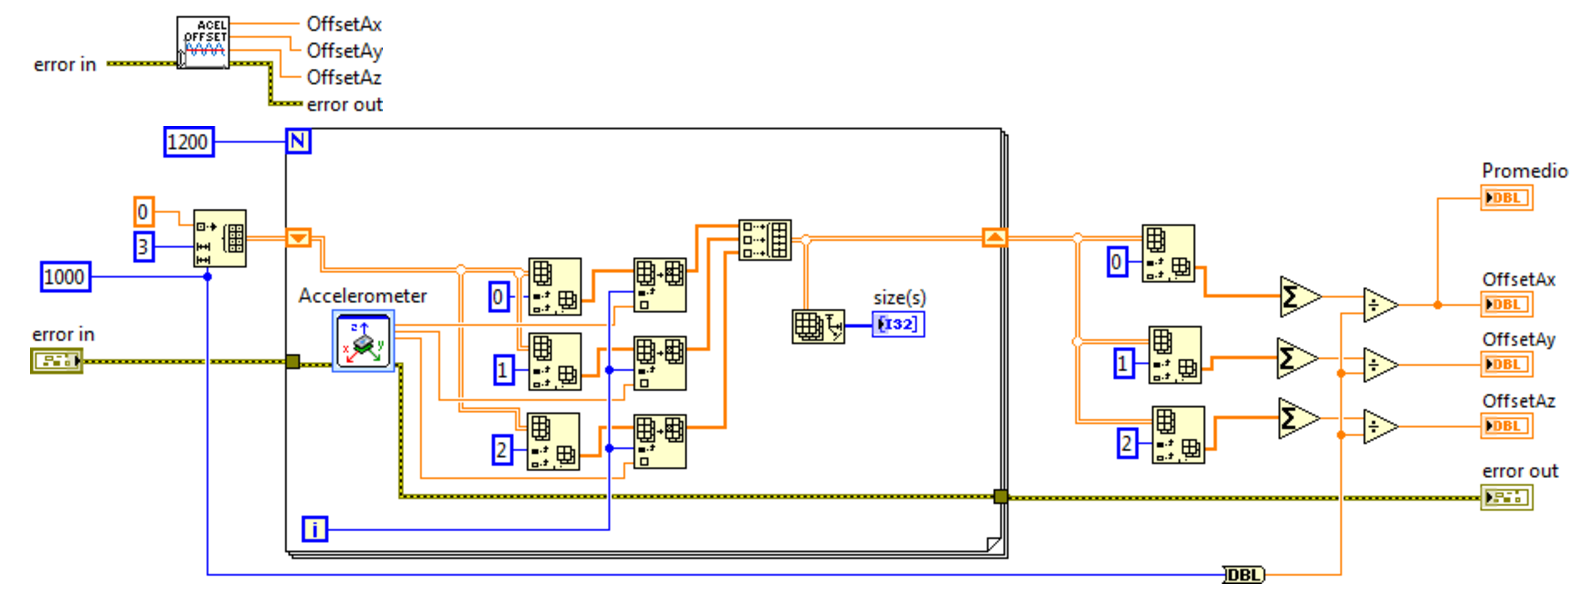
\includegraphics[scale=0.8]{ConfigAcelOffset}
\par\end{raggedright}
\caption{Calculo de offset para acelerómetro.}
\end{figure}

\begin{figure}
\begin{centering}
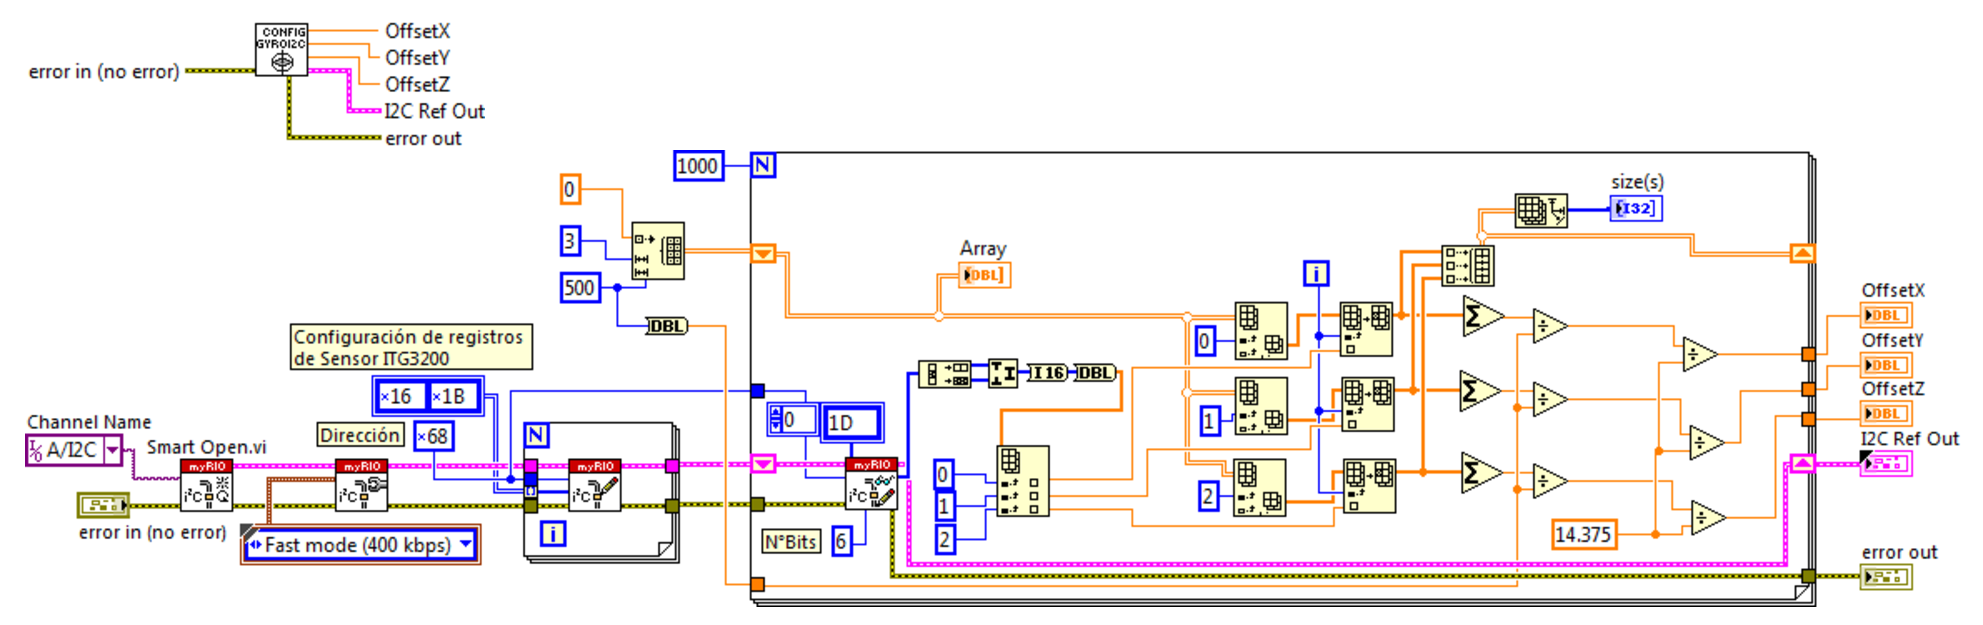
\includegraphics[scale=0.8]{ConfigGyroI2C}
\par\end{centering}
\caption{Configuración de Gyróscopo y cálculo de offset.}
\end{figure}

\begin{figure}
\begin{centering}
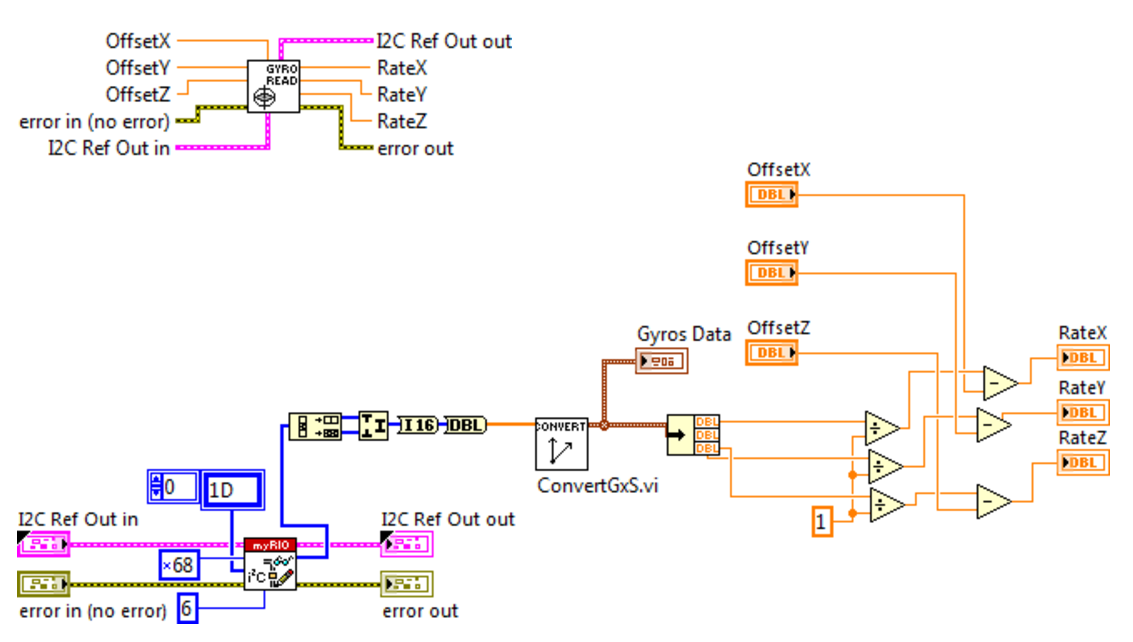
\includegraphics[scale=0.6]{GyroRead}
\par\end{centering}
\caption{}
\end{figure}

\begin{figure}
\begin{centering}
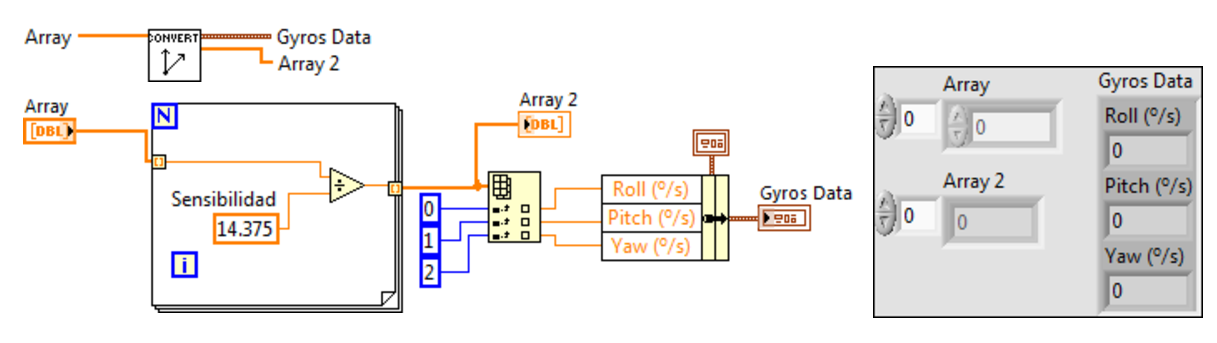
\includegraphics[scale=0.8]{ConvertGxS}
\par\end{centering}
\caption{Conversión de medida de gyróscopo a grados por segundo.}
\end{figure}

\begin{figure}
\begin{centering}
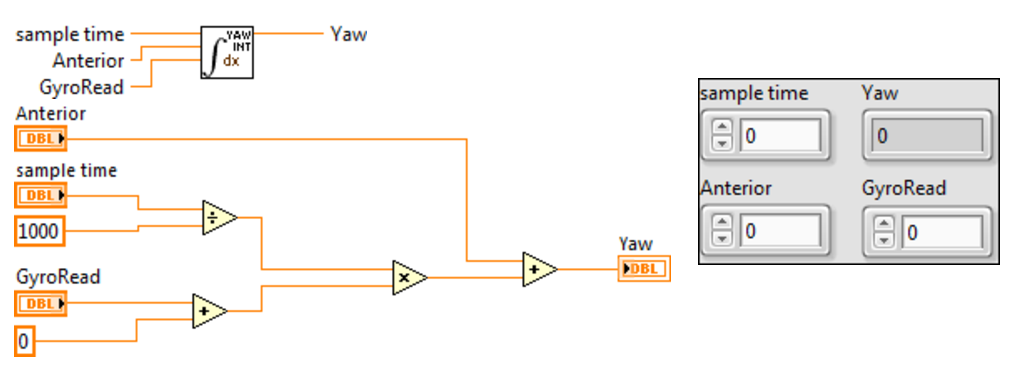
\includegraphics[scale=0.8]{Yaw__integral}
\par\end{centering}
\caption{Cálculo de integral de velocidad en eje Z para ángulo Yaw.}
\end{figure}

\begin{figure}
\begin{centering}
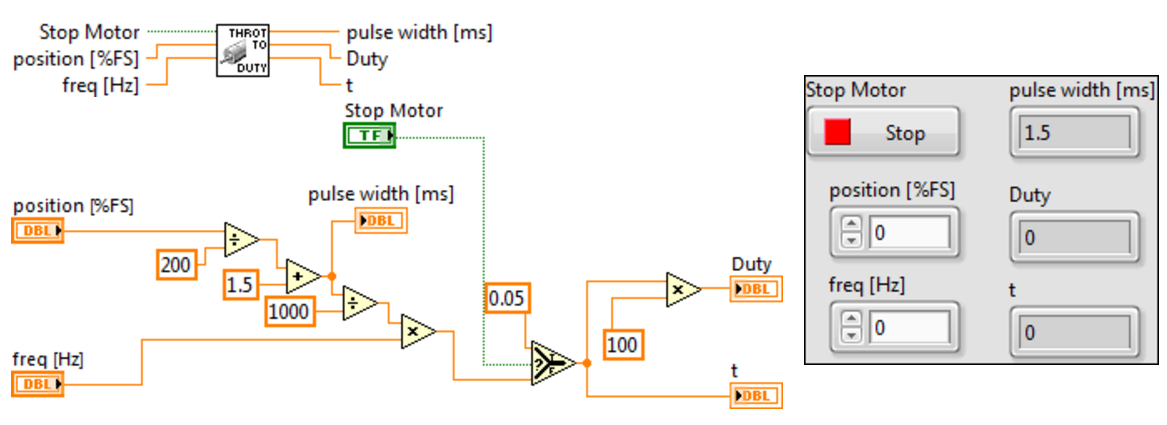
\includegraphics[scale=0.8]{ThrottleToDuty}
\par\end{centering}
\caption{transformación de acelerador a ciclo de trabajo para calibración de motores.}
\end{figure}

\begin{figure}
\begin{centering}
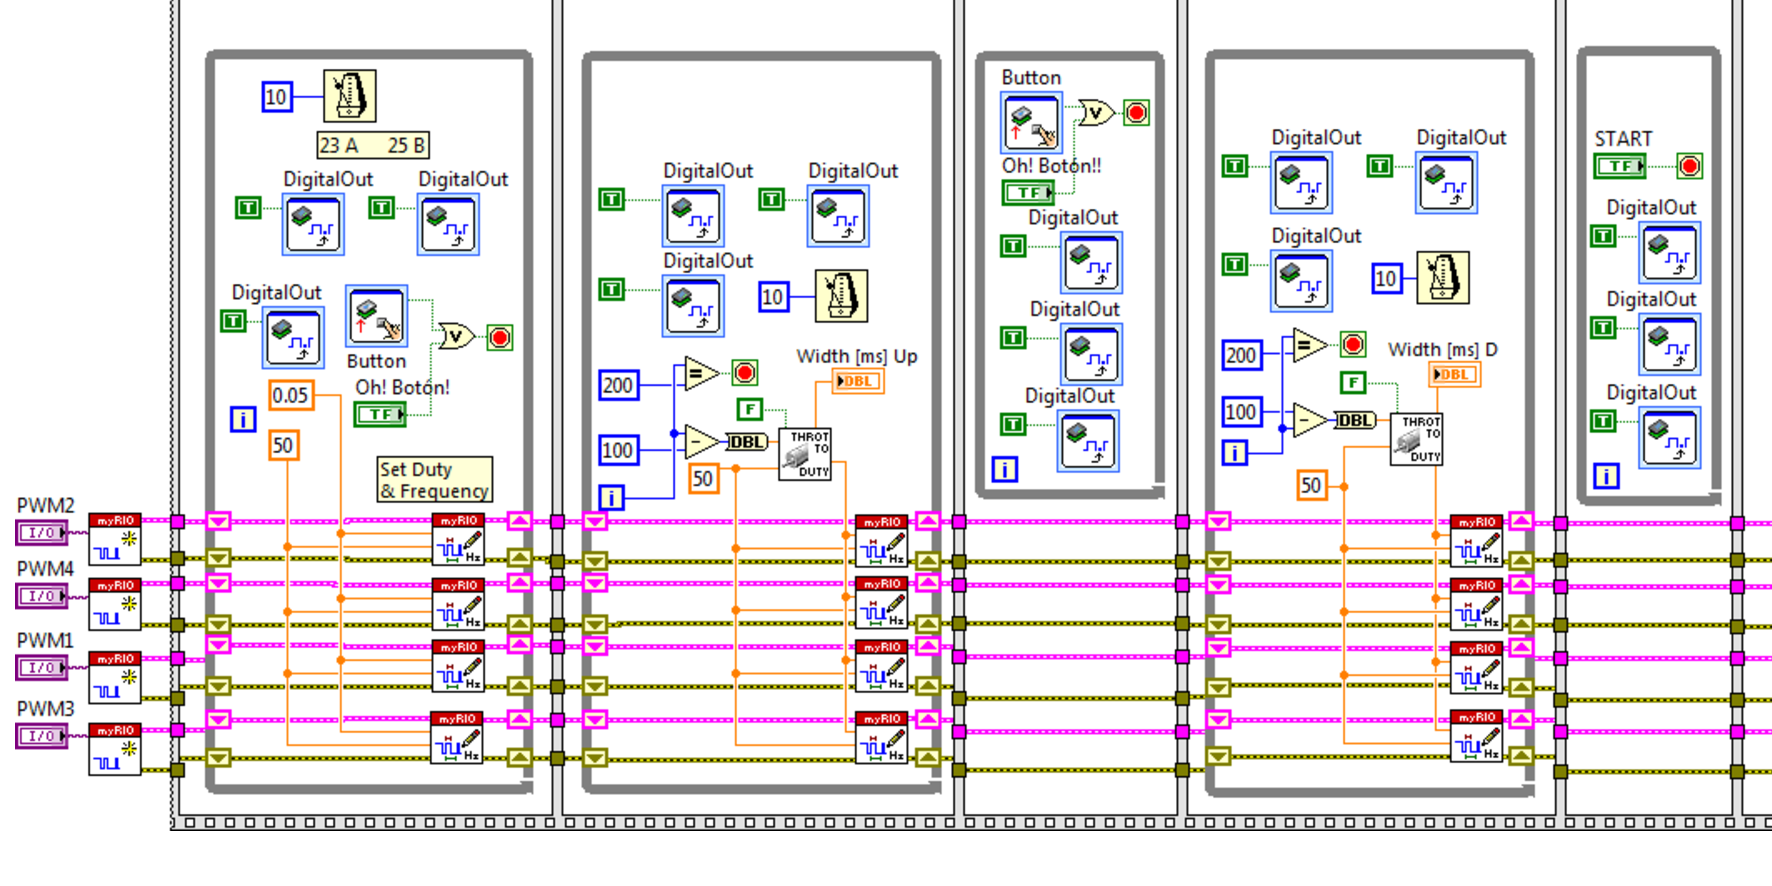
\includegraphics[scale=0.7]{Calibre}
\par\end{centering}
\caption{Calibre automático de motores.}
\end{figure}

\begin{figure}
\begin{centering}
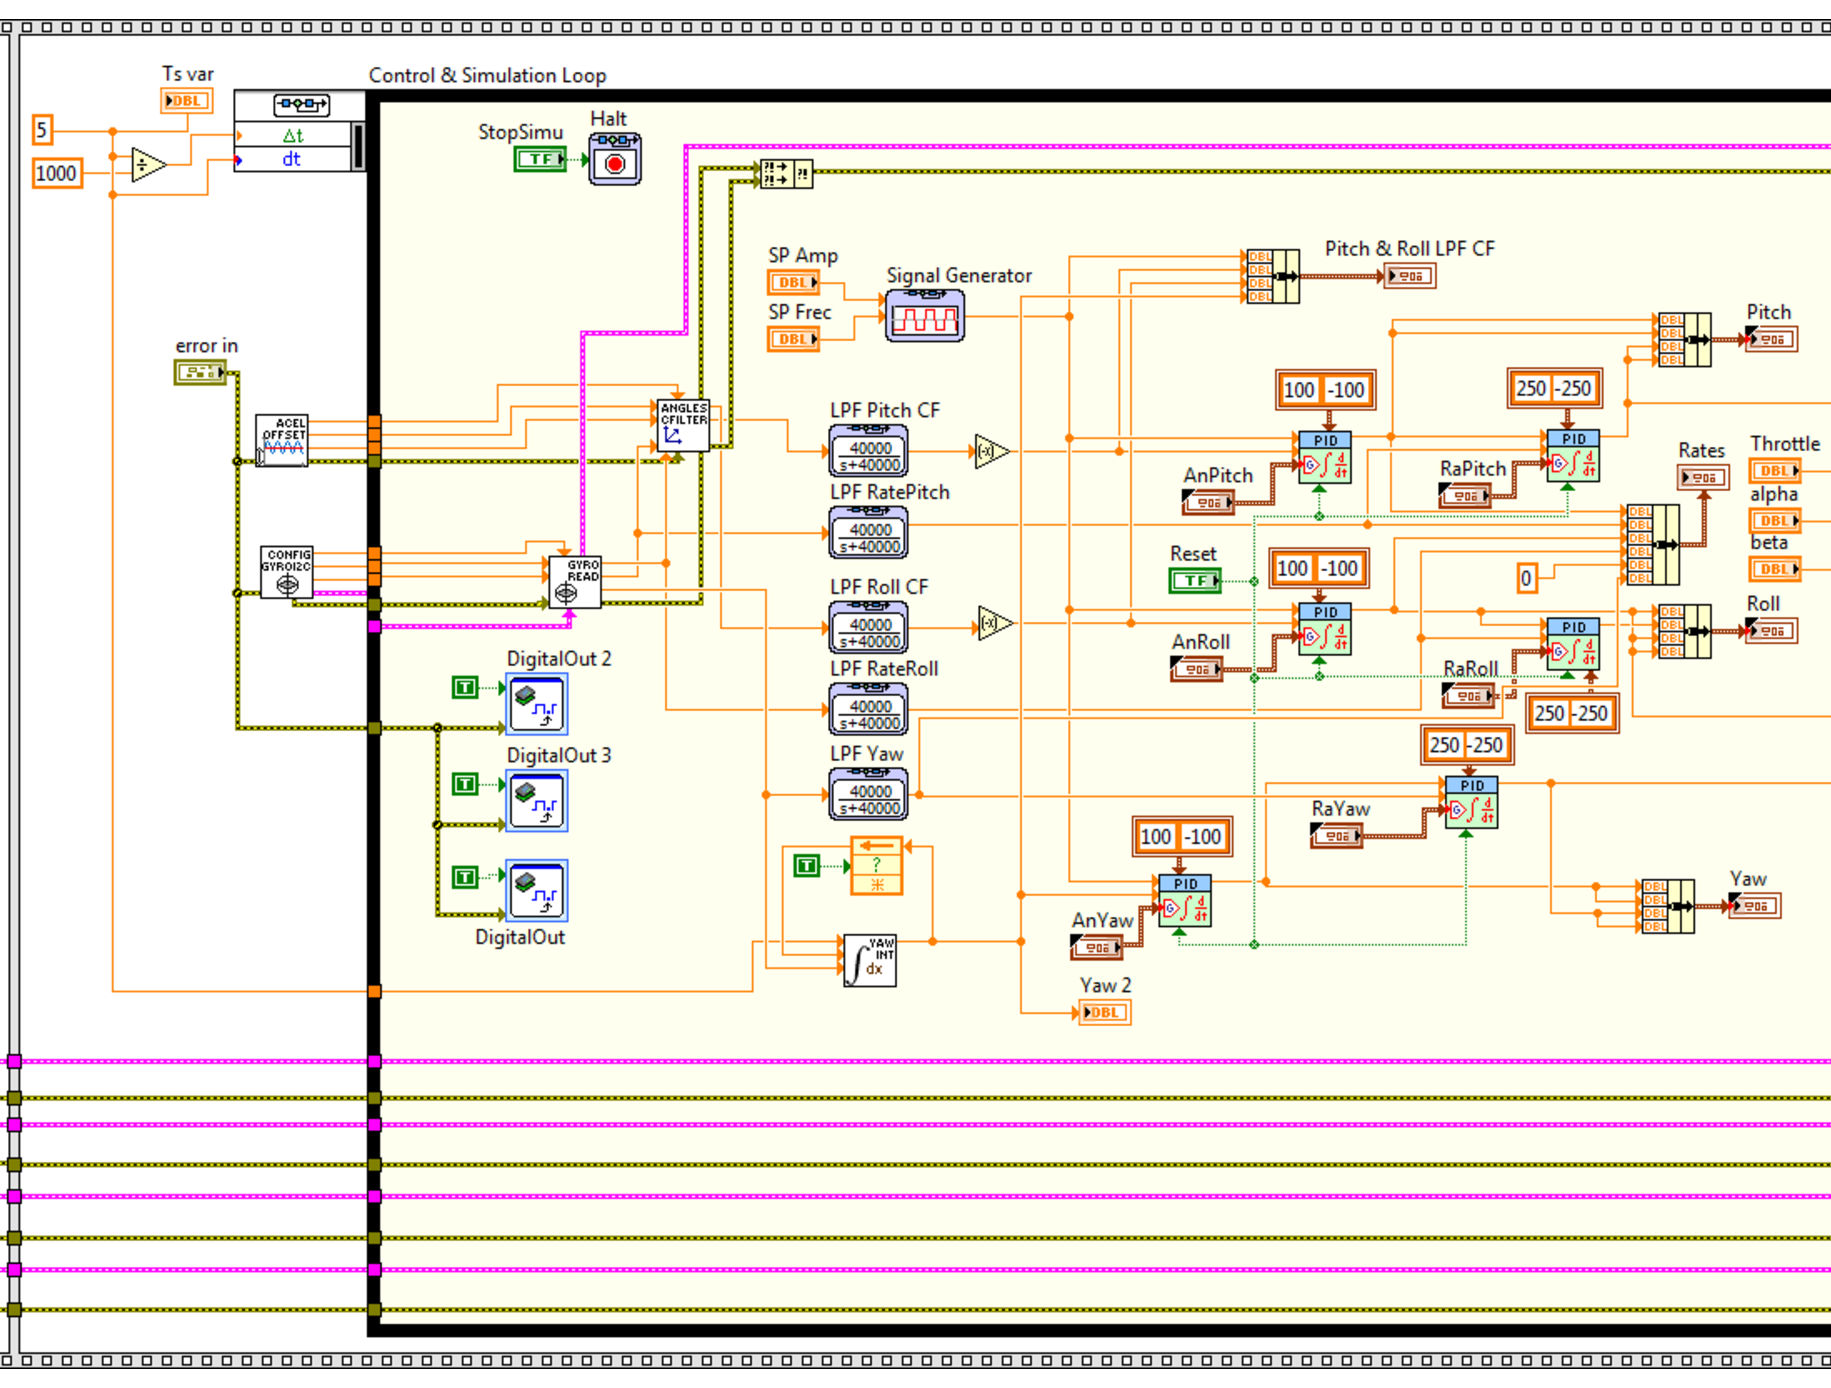
\includegraphics[scale=0.6]{MainLoop1}
\par\end{centering}
\caption{Loop principal parte 1.}
\end{figure}

\begin{figure}
\begin{centering}
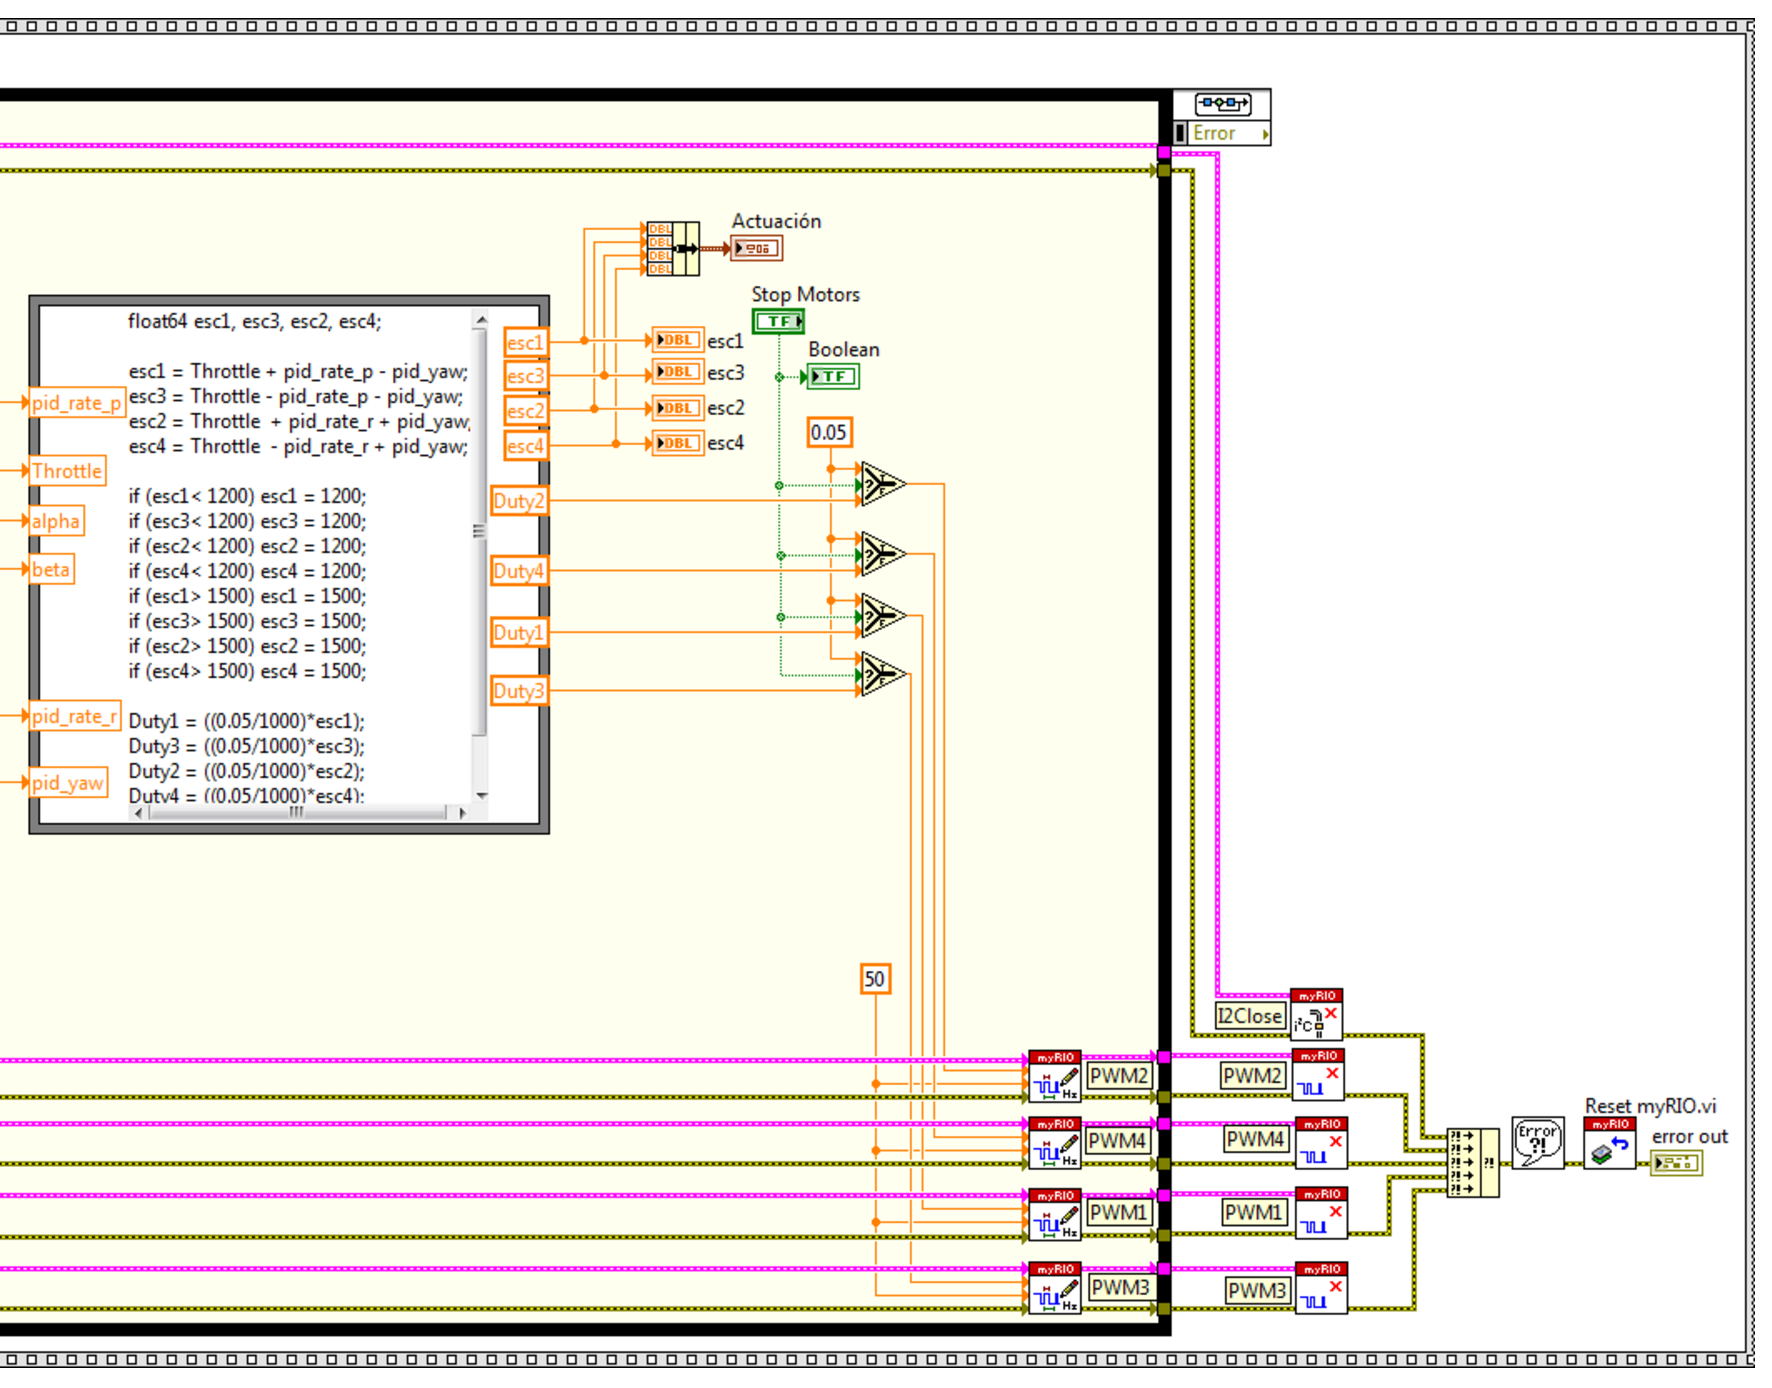
\includegraphics[scale=0.6]{MainLoop2}
\par\end{centering}
\caption{Loop principal parte 2. }
\end{figure}

\begin{figure}
\begin{centering}
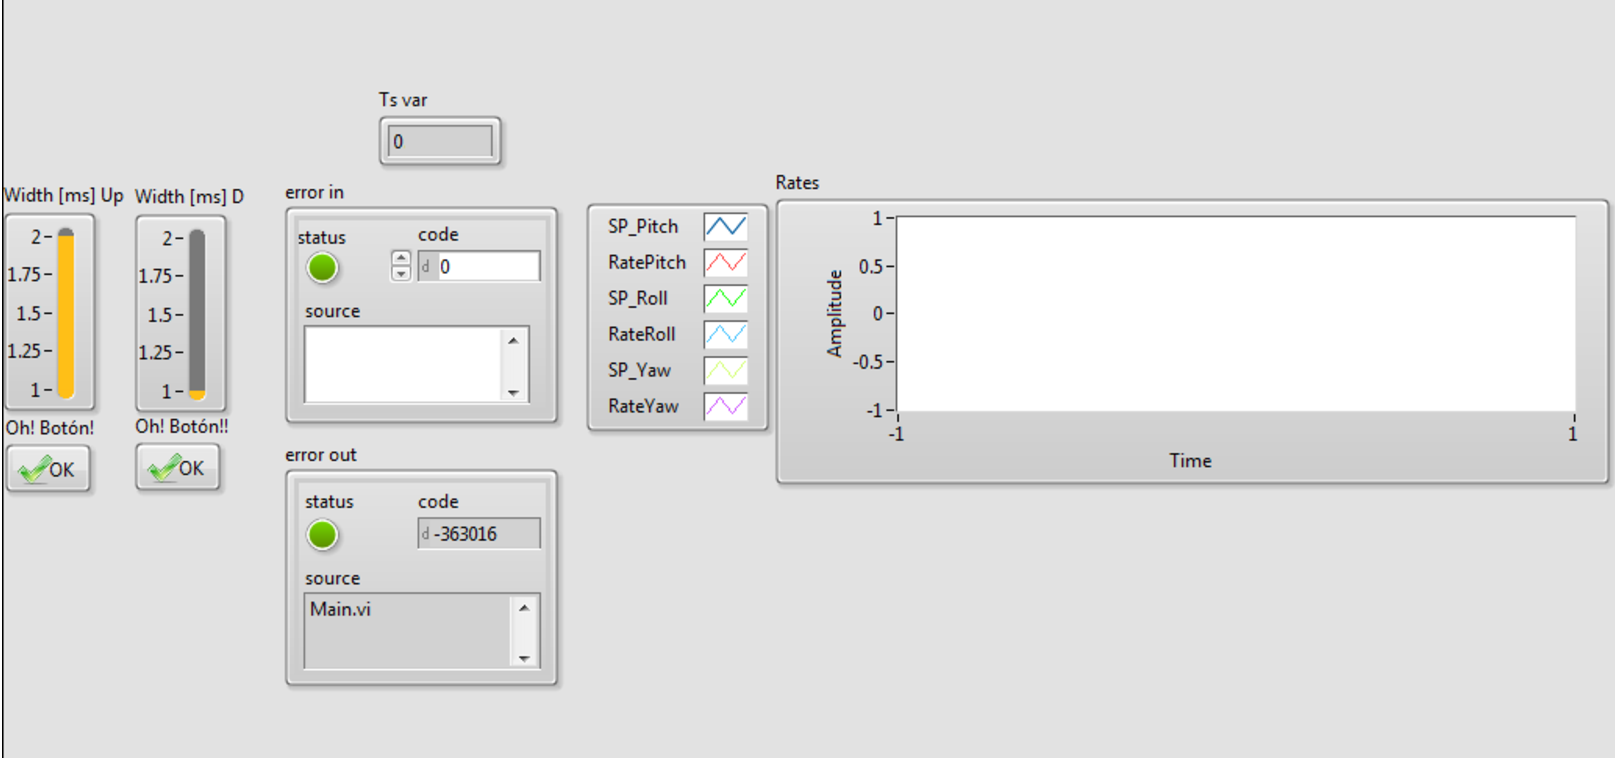
\includegraphics[scale=0.8]{PanelFrontal1}
\par\end{centering}
\caption{Panel frontal principal parte 1.}
\end{figure}

\begin{figure}
\begin{centering}
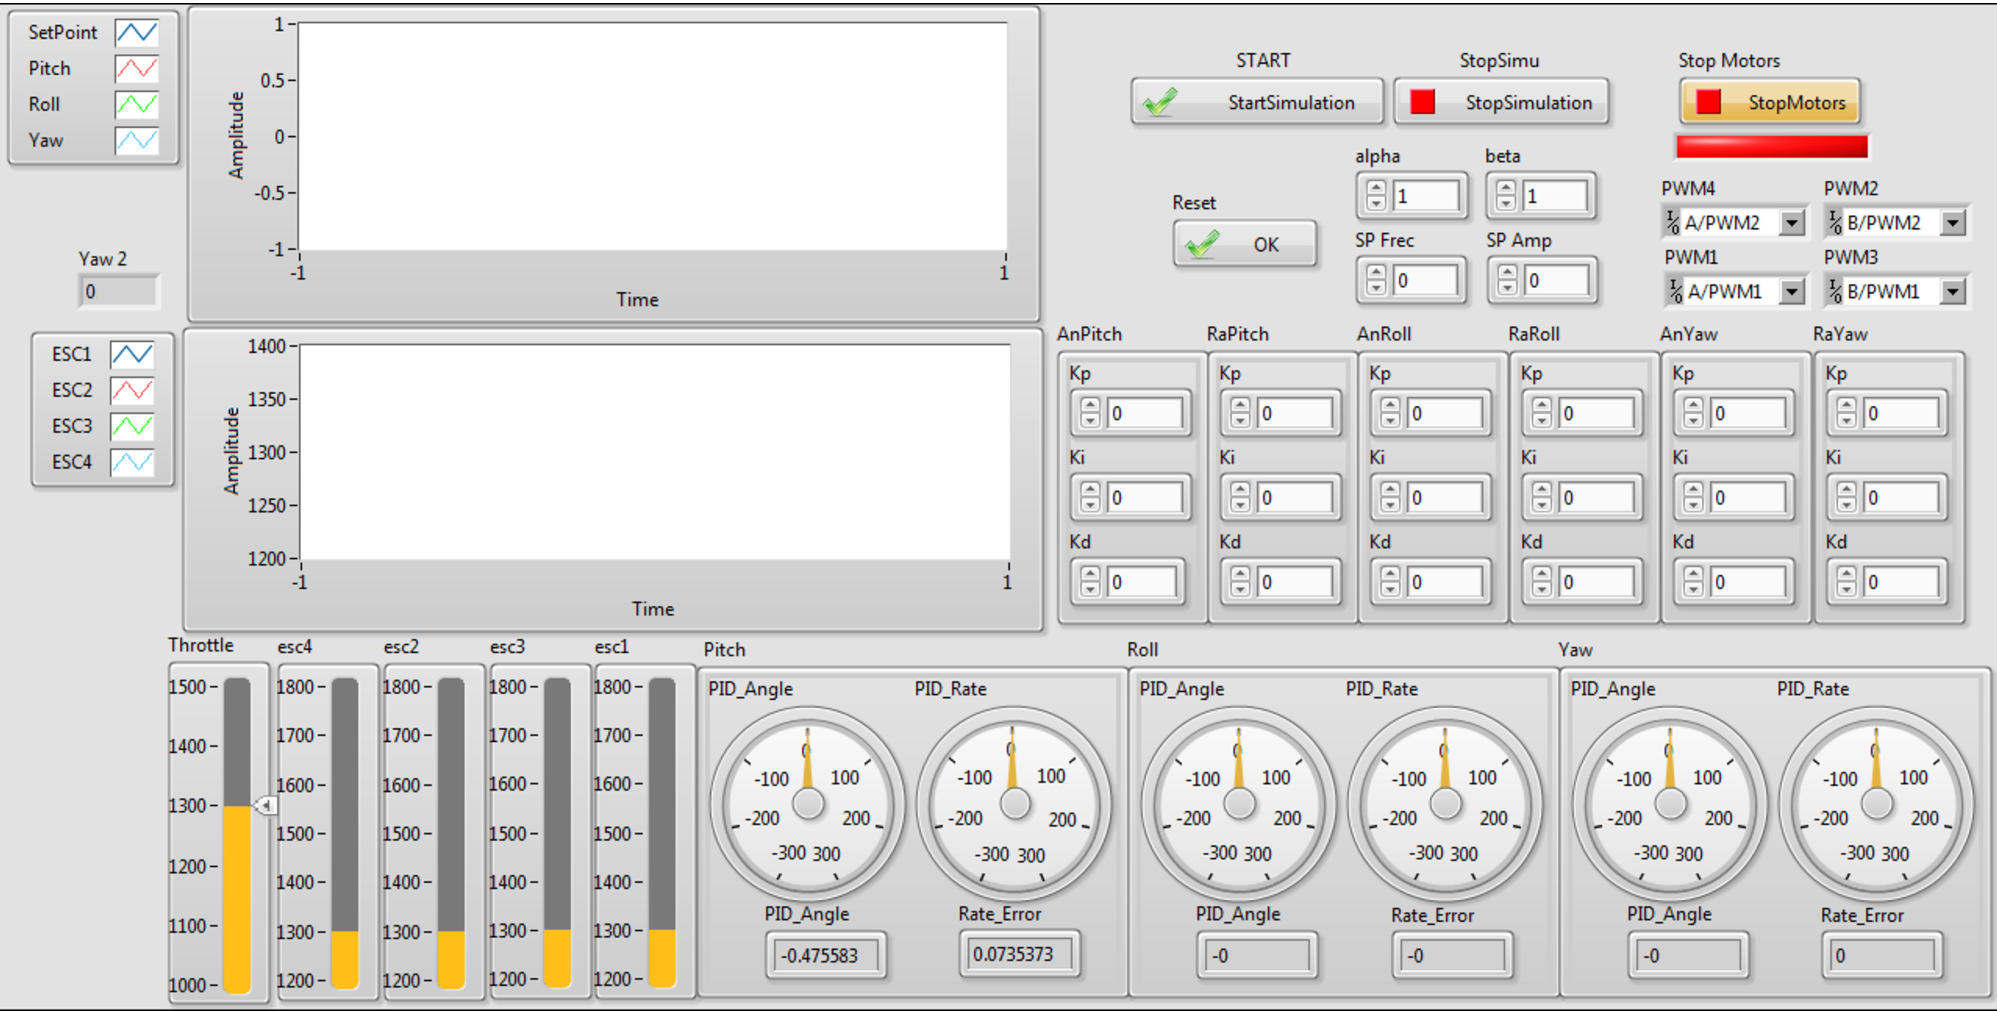
\includegraphics[scale=0.6]{PanelFrontal2}
\par\end{centering}
\caption{Panel frontal principal parte 2.}
\end{figure}

\end{landscape}

\section*{Datos Caracterización de Motores}

\begin{figure}
\begin{centering}
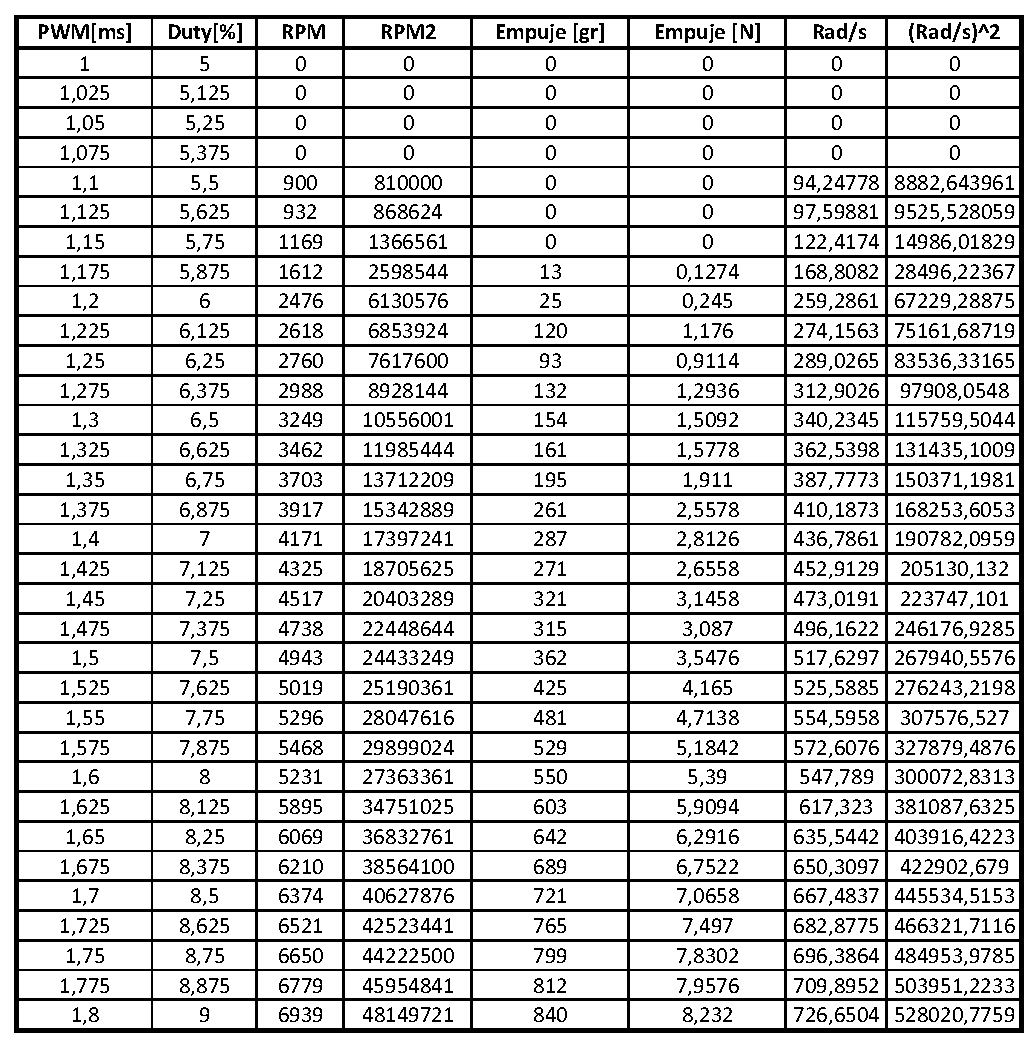
\includegraphics[scale=0.8]{motor1real}
\par\end{centering}
\caption{Mediciones de empuje y velocidad angular para motor 1.}
\end{figure}

\begin{figure}
\begin{centering}
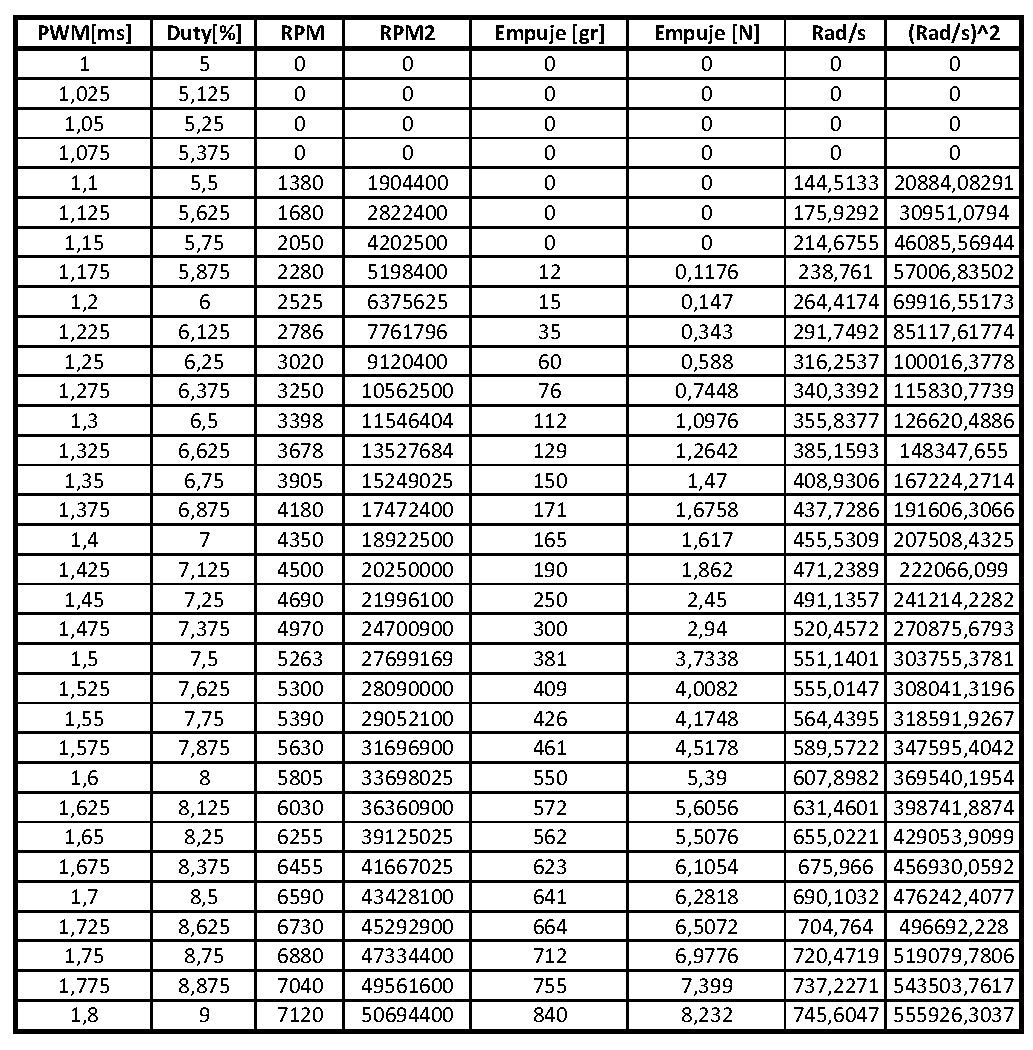
\includegraphics[scale=0.8]{motor2real}
\par\end{centering}
\caption{Mediciones de empuje y velocidad angular para motor 2.}
\end{figure}

\begin{figure}
\begin{centering}
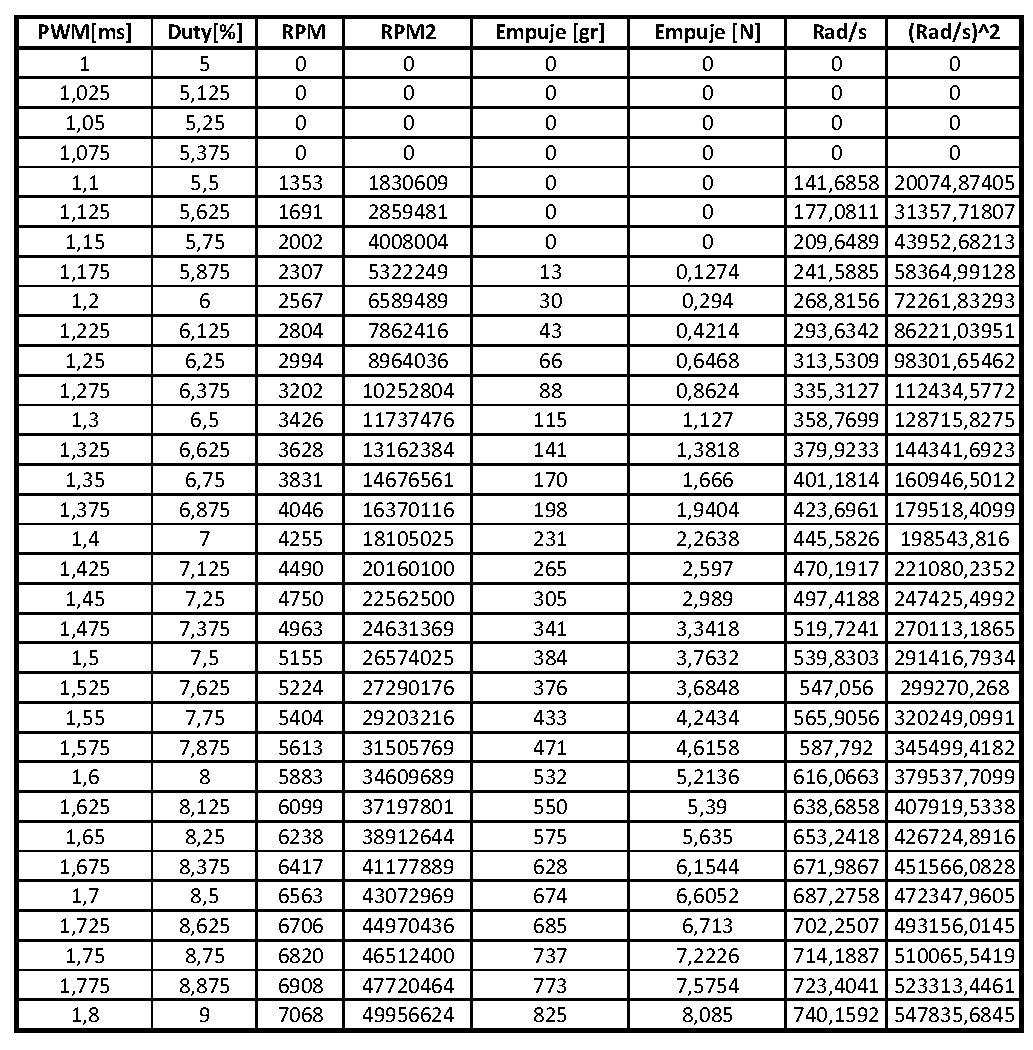
\includegraphics[scale=0.8]{motor3real}
\par\end{centering}
\caption{Mediciones de empuje y velocidad angular para motor 3.}
\end{figure}

\begin{figure}
\begin{centering}
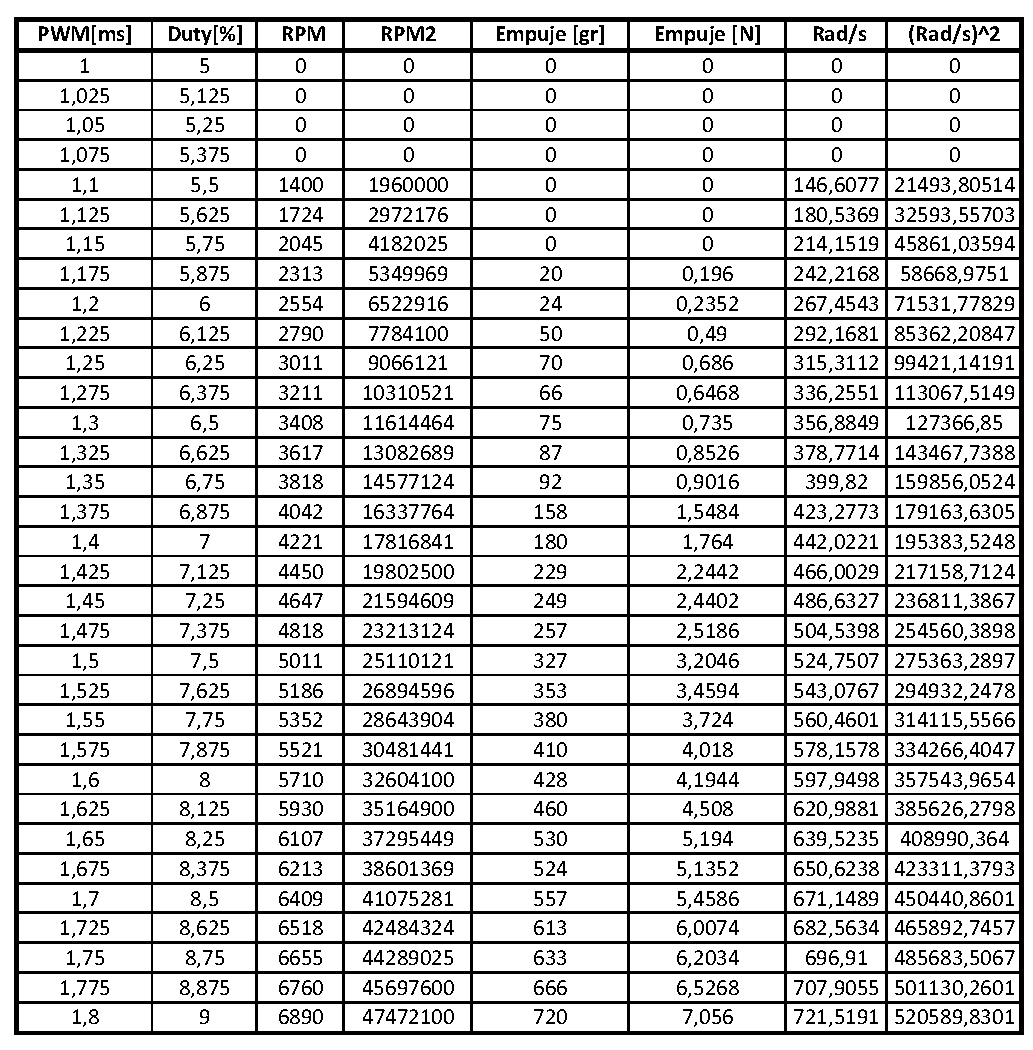
\includegraphics[scale=0.8]{motor4real}
\par\end{centering}
\caption{Mediciones de empuje y velocidad angular para motor 4.}
\end{figure}

\begin{figure}
\begin{centering}
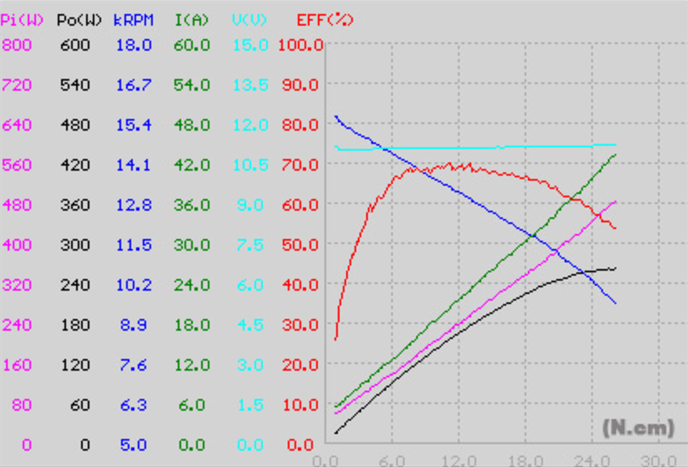
\includegraphics[scale=0.8]{torque}
\par\end{centering}
\caption{Torque v/s velocidad angular.}
\end{figure}

\end{document}